
\section{Teorema de estabilidad}\label{sec:teorema}
En esta sección introduciremos el \emph{teorema de estabilidad de los diagramas de persistencia}, y profundizaremos en su demostración siguiendo \cite{Cohen-Steiner2007}. Primero estudiaremos la estabilidad para la \emph{distancia de Hausdorff}, y después, reforzaremos el resultado estudiando la estabilidad con la \emph{distancia bottleneck}.
\subsection{Proposición del teorema}
El teorema de estabilidad nos va a garantizar la robustez de los diagramas de persistencia. Dicho de otro modo, que ``pequeñas'' perturbaciones en las funciones, dan lugar a diagramas de persistencia ``cercanos''. Así pues, primero precisaremos el concepto de cercanía entre funciones y diagramas de persistencia.

Sean $X$ e $Y$ dos diagramas de persistencia. Recordamos que $X$ e $Y$ son dos multiconjuntos de puntos del plano extendido $\overline{\mathbb{R}}^2$, constituidos por un número finito de puntos sobre la diagonal, y por los puntos de la diagonal con multiplicidad infinito. 

\begin{definition}
Sean los puntos $p=(p_1, p_2)$ y $q=(q_1,q_2)$ en $\overline{\mathbb{R}}^2$. Entonces, la distancia infinito entre los puntos es:
\[
d_\infty(p, q)=\norm{p-q}_\infty= \max\{\abs{p_1 - q_1}, \abs{p_2-q_2}\}\,.
\]
\end{definition}

\begin{definition}
Sean $f,g: \mathbb{X} \to \mathbb{R}$ dos funciones continuas. Entonces, la distancia infinito entre las funciones es:
\[
d_\infty(f, g)=\norm{f-g}_\infty= \sup_{x\in \mathbb{X}}\ \abs{f(z) - g(x)}\,.
\]
\end{definition}

Definiremos las distancias Hausdorff y bottleneck sobre multiconjuntos (diagramas de persistencia en nuestro caso) de la siguiente forma
\begin{definition}
La \emph{distancia Hausdorff} y la \emph{distancia bottleneck} entre $X$ e $Y$ son, respectivamente
\begin{gather*}
H(X, Y) = \max\left\{ \adjustlimits\sup_{x\in X} \inf_{y\in Y} \norm{x-y}_\infty, \adjustlimits\sup_{y\in Y} \inf_{x\in X} \norm{y-x}_\infty \right\},\ \\
W_\infty(X, Y) = \adjustlimits\inf_{\eta: X \to Y} \sup_{x\in X} \norm{x-\eta(x)}_\infty
\end{gather*}
siendo $\eta: X \to Y$ las biyecciones de $X$ a $Y$.
\end{definition}
Las biyecciones entre dos diagramas de persistencia generan tres tipos de emparejamientos:
\begin{itemize}
	\item Ambos puntos fuera de la diagonal.
	\item Un punto fuera de la diagonal y otro en la diagonal.
	\item Ambos puntos en la diagonal.
\end{itemize}
Se puede observar que los puntos que determinar en mayor escala la distancia bottelneck son los del primer tipo, y los que menor importancia tienen son los del último tipo, ya que completarán el emparejamiento sin afectar en la distancia.

\begin{remark}
Debido a que la distancia bottleneck satisface una restricción adicional respecto a la distancia Hausdorff, es decir, la biyección entre los puntos; entonces, se cumple $H(X, Y) \leq W_\infty(X, Y)$.
\end{remark}

\begin{theorem}[Teorema de estabilidad para funciones tame]\label{th:estabilidadTame}
Sea $\mathbb{X}$ un espacio topológico triangulable y sea $f,g: \mathbb{X} \to \mathbb{R}$ dos funciones tame continuas. Entonces, para cada dimensión $k$, la distancia bottleneck entre los diagramas de persistencia esta acotada por la distancia $L_\infty$ entre las funciones, es decir,
\[
W_\infty(\text{\rm Dgm}(f), \text{\rm Dgm}(g)) \leq \norm{f-g}_\infty\,.
\]
\end{theorem}

Luego, se garantiza que los diagramas de persistencia son estables bajo perturbaciones de baja amplitud. Este resultado se puede observar gráficamente en la figura \ref{ref:ejEstabilidad}, donde se observa que los valores críticos ``superfluos'' de la función perturbada definen puntos en el diagrama muy próximos a la diagonal, y los valores críticos ``relevantes'' definen puntos muy próximos a los puntos del diagrama asociados a la función original.

\begin{figure}[!ht]
\centering
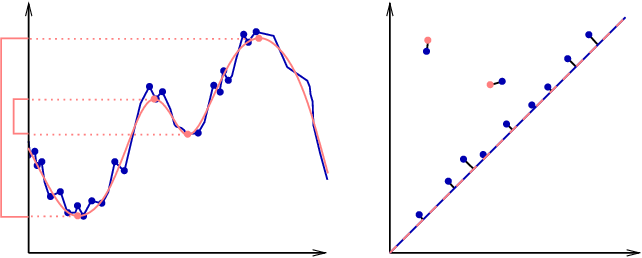
\includegraphics[width=0.8\textwidth]{include/figuras/estabilidadEj.png} 
\caption{A la izquierda se muestran dos funciones cercanas, una con muchos valores críticos y otra con cuatro. A la derecha se muestran los diagramas de persistencia superpuestos, con la biyección que da lugar a la distancia bottleneck. Fuente: \cite{Cohen-Steiner2007}}
\label{ref:ejEstabilidad}
\end{figure}  

\subsection{Estabilidad para la distancia Hausdorff}
Partiremos de la demostración de la estabilidad con la distancia Hausdorff, que sigue sigue así

\begin{theorem}[Teorema de estabilidad con la distancia Hausdorff para funciones tame]
Sea $\mathbb{X}$ un espacio topológico triangulable y sea $f,g: \mathbb{X} \to \mathbb{R}$ dos funciones tame continuas. Entonces, para cada dimensión $k$, la distancia Hausdorff entre los diagramas de persistencia esta acotada por la distancia $L_\infty$ entre las funciones, es decir,
\[
H(\text{\rm Dgm}(f), \text{\rm Dgm}(g)) \leq \norm{f-g}_\infty\,.
\]
\end{theorem}

\subsubsection*{Relaciones entre cuadrantes superiores izquierdos}
Primero estudiaremos la relación entre las multiplicidades de los cuadrantes superiores izquierdos de dos diagramas de persistencia.

\begin{proposition}
Sean $f,g: \mathbb{X} \to \mathbb{R}$ dos funciones tame continuas. Si denotamos $\epsilon = \norm{f-g}_\infty$, entonces $f^{-1}(-\infty,x]\subseteq g^{-1}(-\infty, x+\epsilon]$ para todo $x \in \mathbb{R}$
\end{proposition}

\begin{proof}
Sea $y \in \mathbb{X}$ tal que $y \in f^{-1}(-\infty,x]=\{x\in \mathbb{X} \mid f(x) \in (-\infty,x]\}$. Como $\norm{f-g}_\infty= \sup_{x\in \mathbb{X}}\ \abs{f(z) - g(x)} = \epsilon$, entonces
\[
\abs{f(y)-g(y)}<\epsilon \Rightarrow g(y)\in (-\infty, x+\epsilon] \Rightarrow y \in g^{-1}(-\infty, x+\epsilon]\,.
\]
\end{proof}

Denotamos la aplicación inducida por esta inclusión por $\varphi_x:F_x \to G_{x-\epsilon}$. La inclusión análoga, $g^{-1}(-\infty,x]\subseteq f^{-1}(-\infty, x+\epsilon]$, induce la aplicación $\psi_x: G_x \to F_{x+\epsilon}$. Sea $b<c$, estas dos aplicaciones dan lugar a los siguientes diagramas conmutativos:

% https://tikzcd.yichuanshen.de/#N4Igdg9gJgpgziAXAbVABwnAlgFyxMJZABgBpiBdUkANwEMAbAVxiRADEB9YAIwFoAOgJhpsDAgF8QE0uky58hFACZyVWoxZsuwAMYBqISLGTpskBmx4CRAMxrq9Zq0QduPQ8NFZxYKTLkrRSIAVgcNZ21uAyNvX39zSwUbFDJldSctVwBxdwTA5KVkVXTHTRcQXL18i3lrIvtSiKzKvLMC+tDSJsyKqp4JAD1q6XUYKABzeCJQADMAJwgAWyQyEBwIJABGMsjXWfdBLxM-YZjjn1NqBjoeGAYABTrg1wYYWZx2kAXl1eoNpAAFl2LSE9HmaAAFlhDrETlJrrd7k8gikQPMsBNIZ8At9FitEKp1ptEPZmhUDrxPMZLqc9NS4lcQDc7o9nmi3h8vj8CcDiUgwuS2BM8mcEcykWzUUpme8ceYeQL-iSdkLXEJvJxdCBEayUYU2BisfK5vikAA2ZVIIm9Nga7CcHg6iV69kyzkmvG-RCW-mIADsIIqIt4QxGuuRbrYHu5ZoDVtJQbtAk12ojUoNriN2NGEiAA
\[\begin{tikzcd}
F_{b-\epsilon} \arrow[rr, "f_{b-\epsilon}^{c+\epsilon}"] \arrow[dd, "\varphi_{b-\epsilon}"'] &  & F_{c+\epsilon}              & F_{b+\epsilon} \arrow[rr, "f_{b+\epsilon}^{c+\epsilon}"] &  & F_{c+\epsilon}                  \\
                                                                                             &  &                             &                                                          &  &                                 \\
G_{b} \arrow[rr, "g_{b}^{c}"]                                                                &  & G_{c} \arrow[uu, "\psi_c"'] & G_{b} \arrow[uu, "\psi_b"] \arrow[rr, "g_{b}^{c}"]       &  & G_{b}^{c} \arrow[uu, "\psi_c"']
\end{tikzcd}
\]
Es un diagrama conmutativo, ya que como las función inclusión conmutan, entonces también lo hacen sus aplicaciones inducidas. 

Del primer diagrama tenemos que $f_{b-\epsilon}^{c+\epsilon}=\psi_{c} \circ g_{b}^{c} \circ \varphi_{b-\epsilon}$. Sea $\xi \in F_{b-\epsilon}^{c+\epsilon}=\text{im } f_{b-\epsilon}^{c+\epsilon}$, de forma que $\xi = f_{b-\epsilon}^{c+\epsilon}(\eta)$ para un $\eta \in F_{b-\epsilon}$. Luego, $\xi = \psi_c(\zeta)$, con $\zeta = g_{b}^{c}(\varphi_{b-\epsilon}(\eta)) \in G_{b}^{c}$, por tanto $F_{b-\epsilon} \subseteq \psi_{c}(G_{b}^{c})$.

Del segundo diagrama, tenemos que $\psi_{c}(G_{b}^{c})=\psi_{c} \circ g_{b}^{c}(G_b)$, ya que $G_{b}^{c}=\text{im } g_{b}^{c} = g_{b}^{c}(G_b)$. A su vez, se cumple que $\psi_{c} \circ g_{b}^{c}(G_b) = f_{b+\epsilon}^{c+\epsilon} \circ \psi_{b}(G_b) \subseteq F_{b+\epsilon}^{c+\epsilon} \Rightarrow \psi_{c}(G_{b}^{c}) \subseteq F_{b+\epsilon}^{c+\epsilon}$.

Así pués, se cumple:
\begin{equation}\label{eq:relCuadrantes}
F_{b-\epsilon}^{c+\epsilon} \subseteq \psi_{c}(G_{b}^{c}) \subseteq F_{b+\epsilon}^{c+\epsilon}\,.
\end{equation}

De manera análoga podemos demostrar que se cumple que
\[
 G_{b-\epsilon}^{c+\epsilon} \subseteq \varphi_{c}(F_{b}^{c}) \subseteq G_{b+\epsilon}^{c+\epsilon}
\]
intercambiando $F_{x}$ y $G_{y}$ en los diagramas y sustituyendo las aplicaciones inducidas correctamente.
	
\begin{theorem}[Fórmula de las dimensiones \cite{AlgebraLineal}]\label{ref:FormulaDim}
Si una aplicación $f: U \to V$ es lineal entonces se cumple que
\[
\text{\rm dim ker } f + \text{\rm dim im } f = \text{\rm dim } U\,. 
\]
\end{theorem}

De la primera inclusión de \ref{eq:relCuadrantes} obtenemos que $\text{dim } F_{b-\epsilon}^{c+\epsilon} \leq \text{dim } \psi_{c}(G_{b}^{c}) \overset{Th.\  \ref{ref:FormulaDim}}{\leq} \text{dim } G_{b}^{c}$. Aplicando el \emph{Lema del $k$-Triángulo} a la anterior desigualdad y denotando a los cuadrantes superiores izquierdos como $Q = Q_{b}^{c}$ y $Q_\epsilon = Q_{b-\epsilon}^{c+\epsilon}$, se obtiene el siguiente resultado:

\begin{figure}[h]
\centering
\begin{tikzpicture}[thick]
    \tikzstyle{point}=[circle,thick,draw=black,fill=black,inner sep=0pt,minimum width=4pt,minimum height=4pt]
        	\tikzstyle{point1}=[circle,thick,draw=black,fill=white,inner sep=0pt,minimum width=4pt,minimum height=4pt]
    
    \draw[->] (-2.5,-2) -- (3.5,-2) node[right] {$x$};
    \draw[->] (2,-2.5) -- (2,2.5) node[above] {$y$};

    \begin{scope}[xshift=2cm,yshift=-2cm]
    	\coordinate (a) at (-1, 1.5);
    	\coordinate (ax) at (-1,0);
    	\coordinate (ay) at (0, 1.5);
    	\coordinate (b) at (-4.5, 1.5);
    	\coordinate (c) at (-4.5, 4.5);
    	\coordinate (d) at (-1,  4.5);
    	
    	\coordinate (a1) at (-2, 2.5);
    	\coordinate (a1x) at (-2, 0);
    	\coordinate (a1y) at (0, 2.5);
    	\coordinate (b1) at (-4.5, 2.5);
    	\coordinate (d1) at (-2,  4.5);
    	
    	\coordinate (p1) at (-1.3,  3);
    	\coordinate (p2) at (-4,  3.6);
		\coordinate (p3) at (-2.8,  4.1);
		\coordinate (p4) at (-3.2,  1.8);
		\coordinate (p5) at (-3,  3.2);
    \end{scope}


    \draw[greeo,fill=greeo,opacity=0.6] (a) -- (b) -- (c)--(d) -- cycle;
    \draw[redp,fill=redp] (a1) -- (b1) -- (c)--(d1) -- cycle;
	\draw[thick] (a) -- (b);
	\draw[thick] (a) -- (d);
	\draw[thick] (a1) -- (b1);
	\draw[thick] (a1) -- (d1);
	\draw[thick,dashed,opacity=0.6] (ay) -- (a);
	\draw[thick,dashed,opacity=0.6] (ax) -- (a);
	\draw[thick,dashed,opacity=0.6] (a1y) -- (a1);
	\draw[thick,dashed,opacity=0.6] (a1x) -- (a1);
    
	\node ()[point] at (a) {};
	\node ()[point] at (a1) {};
	\node [below=0.1cm of a1x] {$b-\epsilon$};
	\node [below=0.1cm of ax] {$b$};
	\node [right=0.1cm of a1y] {$c+\epsilon$};
	\node [right=0.1cm of ay] {$c$};
	\node ()[point1] at (p1){};
	\node ()[point1] at (p2){};
	\node ()[point1] at (p3){};
	\node ()[point1] at (p4){};
	\node ()[point1] at (p5){};
\end{tikzpicture}
\caption{Representación del \emph{Lema del cuadrante}}
\label{ref:lemaCuadranteDib}
\end{figure}

\begin{lemma}[Lema del cuadrante]
$\#(\text{\rm Dgm}(f) \cap Q_\epsilon) \leq \#(\text{\rm Dgm}(g) \cap Q)\,.$
\end{lemma}

\begin{proof}
Si $b$ y $c$ no son valores críticos homológicos de $g$ y $b-\epsilon$, $c+\epsilon$ no son valores críticos homológicos de $f$, entonces por el Lema del $k$-Triángulo
\[
\#(\text{\rm Dgm}(g) \cap Q)= \beta_{b}^{c} = \text{dim } G_{b}^{c} 
\text{ y }
\#(\text{\rm Dgm}(f) \cap Q_\epsilon)= \beta_{b-\epsilon}^{c+\epsilon} = \text{dim } F_{b-\epsilon}^{c+\epsilon} \,.
\]
Y como se tiene $\text{dim } F_{b-\epsilon}^{c+\epsilon} \leq \text{dim } G_{b}^{c}$, entonces $\#(\text{\rm Dgm}(f) \cap Q_\epsilon) \leq \#(\text{\rm Dgm}(g) \cap Q)\,.$

En el caso que los puntos $b$ y $c$ sean valores críticos homológicos de $g$ y $b-\epsilon$, $c+\epsilon$ son valores críticos homológicos de $f$, entonces podemos engordar los cuadrantes una cantidad $0<\delta<\epsilon$, tal que
\[
\#(\text{\rm Dgm}(f) \cap Q_\epsilon)=\#(\text{\rm Dgm}(f) \cap Q_{b-\epsilon+\delta}^{c+\epsilon-\delta}) 
\text{ y }
 \#(\text{\rm Dgm}(g) \cap Q)=\#(\text{\rm Dgm}(g) \cap Q_{b+\delta}^{c-\delta})\,,
\]
siendo estas nuevas coordenadas distintas de los valores críticos de $f$ y $g$ respectivamente.
\end{proof}

Este lema nos garantiza que la multiplicidad total de $\text{Dgm}(g)$ en el cuadrante superior izquierda con vértice en el punto $(b, c)$ esta acotada inferiormente por la multiplicidad total de $\text{Dgm}(f)$ en el cuadrante superior izquerda reducida por $\epsilon$. Esto se puede observar en la figura \ref{ref:lemaCuadranteDib}.

\subsubsection*{Regiones como subespacios vectoriales}
\begin{sloppypar}
Sin embargo, el \emph{Lema del cuadrante} no es lo suficientemente fuerte para nuestros propósitos. Vamos a obtener un resultado similar al \emph{Lema del cuadrante}, pero en este caso para cajas encajadas. Esto se debe a que si se cumple ${H(\text{Dgm}(f), \text{Dgm}(g)) \leq \norm{f-g}_\infty = \epsilon}$, entonces para todo punto $(x,y) \in \text{Dgm}(f)$ debe haber un punto en $\text{Dgm}(g)$ a distancia menor o igual que $\epsilon$. Lo que significa que debe haber un punto $q \in \text{Dgm}(g)$ dentro del cuadrado $[x-\epsilon, x+\epsilon]\times[y-\epsilon, y+\epsilon]\,,$ \cite{presentacionEstabilidad}.
\end{sloppypar}

Para definir estas regiones introduciremos subespacios vectoriales de $\overline{\mathbb{R}}^2$ y haremos uso del \emph{Lema del $k$-triángulo} para poder expresar sus dimensiones como la multiplicidad total del diagrama de persistencia en dichas regiones.

Sean $w < x < y <z \in \mathbb{R}$ puntos diferentes a los valores críticos homológicos de $f:\mathbb{X} \to \mathbb{R}$. Recordamos que la dimensión del grupo de homología $F_x$ es igual a la multiplicidad total en el cuadrante superior izquierdo de vértice el punto de la diagonal $(x,x)$, y la dimensión del grupo de persistencia $F_{x}^{y}$ es igual a la multiplicidad total en el cuadrante superior izquierdo de vértice el punto $(x,y)$. Estas regiones se pueden observar en las figuras \ref{ref:regHausdorff}$\,$(a),(b).

\begin{figure}[!ht]
\centering
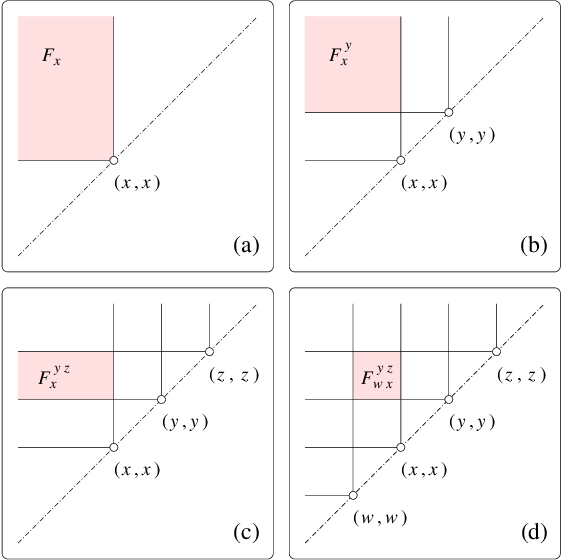
\includegraphics[width=0.6\textwidth]{include/figuras/regionesHausdorffSinComas.png} 
\caption{(a) Grupo de homología del conjunto de subnivel $f^{-1}(-\infty,x]\,.$ (b) Imagen de $F_x$ en $F_y\,.$ (c) Núcleo de la sobreyección $F_{x}^{y} \to F_{x}^{z}\,.$ (d) Cociente de $\tensor*{F}{*_{x}^{y\,}_{}^{z}}$ y $\tensor*{F}{*_{w}^{y\,}_{}^{z}}\,.$ Fuente: \cite{Cohen-Steiner2007}}
\label{ref:regHausdorff}
\end{figure} 

\begin{sloppypar}
Si restringimos $f_{x}^{y}: F_y \to F_z$ al espacio vectorial $F_x^y$ tenemos la epimorfismo ${\tensor*{f}{*_{x}^{y\,}_{}^{z}}:F_{x}^{y} \to F_{x}^{z}}$, ya que todas las clases de homología que están vivas en $x$ y siguen vivas en $z$, deben de seguir vivas en $y<z$. Escribiendo $\tensor*{F}{*_{x}^{y\,}_{}^{z}}$ el núcleo de dicha aplicación, tenemos que $\text{dim } \tensor*{F}{*_{x}^{y\,}_{}^{z}} = \text{dim } F_{x}^{y}-\text{dim } F_{x}^{z}$. Lo que corresponde con la sección marcada en la figura \ref{ref:regHausdorff}$\,$(c).
\end{sloppypar}

Además, podemos observar que se cumple $F_w^y \subseteq F_x^y$, ya que todo elemento de $F_w^y$, el cual es la imagen de un $\xi\in F_w$ por la aplicación $f_w^y$, es también la imagen de $f_w^x(\xi)$ por la aplicación  $f_x^y$. Como consecuencia, $ \tensor*{F}{*_{w}^{y\,}_{}^{z}} \subseteq  \tensor*{F}{*_{x}^{y\,}_{}^{z}}\,$, y por tanto podemos definir el siguiente cociente
\[
\tensor*{F}{*_{w\;}^{y\,}_{x}^{z}}= \dfrac{\tensor*{F}{*_{x}^{y\,}_{}^{z}}}{\tensor*{F}{*_{w}^{y\,}_{}^{z}}}\,.
\]
Al ser un cociente de subespacios vectoriales, su dimensión es la diferencia de los dos núcleos, es decir, $\text{dim } \tensor*{F}{*_{w\;}^{y\,}_{x}^{z}} = \text{dim } \tensor*{F}{*_{x}^{y\,}_{}^{z}}-\text{dim } \tensor*{F}{*_{w}^{y\,}_{}^{z}}\,$. Lo que es quivalente a la multiplicidad total en del diagrama de persistencia en la caja $[w,x]\times [y,z]$; como se puede observar en la figura \ref{ref:regHausdorff}$\,$(d).

\subsubsection*{Relaciones entre cajas encajadas}



\begin{lemma}[Lema de la caja]\label{eq:lemaCaja}
Sean $a < b < c < d \in \mathbb{R}$, $R=[a,b]\times[c,d]$ una caja en $\overline{\mathbb{R}}^2$ y $R_\epsilon=[a+\epsilon,b-\epsilon]\times[c+\epsilon,d-\epsilon]$ la caja obtenida de reducir $R$ en todos sus lados. Entonces se cumple
\[
\#(\text{\rm Dgm}(f) \cap R_\epsilon) \leq \#(\text{\rm Dgm}(g) \cap R)\,.
\]
\end{lemma}

\begin{figure}[!ht]
\centering
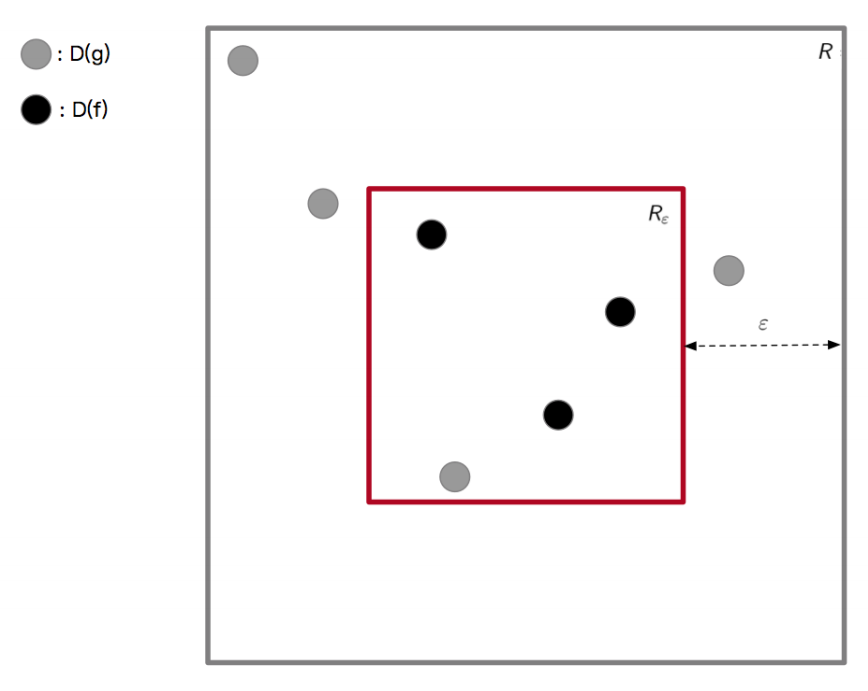
\includegraphics[width=0.5\textwidth]{include/figuras/boxLemma.png} 
\caption{Representación del \emph{Lema de la caja}. Fuente: \cite{presentacionEstabilidad}}
\label{ref:boxLemma}
\end{figure}

Para poder demostrar el \emph{Lema de la caja} primero recordemos el \emph{Segundo teorema de isomorfía}:
\begin{theorem}[Segundo teorema de isomorfía \cite{teoremasIsomorfia}]\label{ref:segThIso}
Sea  $V$ un espacio vectorial y sean $S$ y $T$ dos subespacios de $V$, entonces
\begin{enumerate}
	\item $S + T =\{v\in V \mid v= s+t, s\in S \text{ y } t\in T\}$ es un subespacio de $V$.
	\item $S/(S \cap T) \cong (S+T)/T\,$.
\end{enumerate}

\end{theorem}

\begin{proof}[Demostración del Lema \ref{eq:lemaCaja} (Lema de la caja)]
Podemos asumir sin perder generalidad que $a$, $b$, $c$ y $d$ no son valores críticos homológicos de $g$ y $a+\epsilon$, $b-\epsilon$, $c+\epsilon$ y $d-\epsilon$ no son valores críticos homológicos de $f$. Además consideraremos que $a + \epsilon < b -\epsilon$ y $c + \epsilon < d - \epsilon$, de forma que $R_\epsilon$ este bien definido.

Para el cálculo de las multiplicidades totales dentro de las cajas haremos uso de las dimensiones de los subespacios vectoriales asociados, es decir,
\begin{equation}\label{eq:Mf-F}
\text{dim } \tensor*{F}{*_{a+\epsilon\;}^{c+\epsilon\,}_{b-\epsilon}^{d-\epsilon}} = \#(\text{\rm Dgm}(f) \cap R_\epsilon)\,, 
\end{equation}
\begin{equation}\label{eq:G-Mg}
\text{dim } \tensor*{G}{*_{a\;}^{c\,}_{b}^{d}} = \#(\text{\rm Dgm}(g) \cap R)\,. 
\end{equation}

Para demostrar que $\text{dim } \tensor*{F}{*_{a+\epsilon\;}^{c+\epsilon\,}_{b-\epsilon}^{d-\epsilon}} \leq \text{dim } \tensor*{G}{*_{a\;}^{c\,}_{b}^{d}}$, buscaremos una epimorfismo entre un subespacio vectorial de $\tensor*{G}{*_{a\;}^{c\,}_{b}^{d}}$ a $ \tensor*{F}{*_{a+\epsilon\;}^{c+\epsilon\,}_{b-\epsilon}^{d-\epsilon}} \leq \text{dim }$. Para la construcción de dicha aplicación haremos uso del diagrama conmutativo que se muestra en la figura \ref{ref:diagCon1}, el cual garantizaremos que esta bien definido y que es conmutativo.

\begin{figure}[!ht]
% https://tikzcd.yichuanshen.de/#N4Igdg9gJgpgziAXAbVABwnAlgFyxMJZABgBpiBdUkANwEMAbAVxiRAHEB9YOgXwD1gUXiF6l0mXPkIoATKVlVajFmwBi3OgGoAOjphpsDAgKEBaPQaMnR4kBmx4CReQBYl9Zq0QgNPXfqGWMZgpgDGAVbBNmISjtJErgoeKt6+3ABGFoHWoYJQ2VEhIrH2kk4yyEnu1J6qPn5ZlkHFghHNuSV2DlLOKGQAbClebFw84bx6cEyGMDgwAI4ABACimhO2cb2VA+TD9RyZpsKbZfF9yLtDtalsa8AZE1NMGXBzi0tjj20lSjBQAHN4ERQAAzABOEAAtkh5CAcBAkABGagMOgZGAMAAK5QSPgYMFBOBANxGPlBmkiLRMbSpuVIBQ60VCAF4mJxZKcIdDkdQEUgAMx8ujBNgACwgEAA1iTlGSQOCOSysFzITDEEl4YjEEKQGiMdjcX0FVgAWLiaSDuyBSyKQ9CtS8sB2jlmQyHZ1VTzEHD+RrhaKfBLpbK6mlFTaVaVueqAKx87VwsNsPRBThhPQ0GDgnDcNZ0fhhXgsuAc2X6zE484yPWE4nRtVIeNapBkOUHAHrNoMyY6LM5vOcAtFtmcJHl9GVo01glEr3qtt+3bwkUMcWSmWW8NjpYspZRuwxwUJpDL5M+TN0cFoMVYdOZ7O54CND3M46v4rF0vjhve5t+gB2Lc2EVVxlVlHBV3XENf3VICW39PVJ0NasQNNc1Q1uHxSxtVNsHvPtH0HDJCy6MFG0QeCl1RZCq22NCzQtds0nZMDOwecIewfAdgDWEii1ECheCAA
\[
\begin{tikzcd}
G_{a}^{d} \arrow[rrrrrr, "r_1 = i", hook]                                                                                                           &  &                                                                                                                  &  &                                                                                              &  & G_{b}^{d}                                                                                                               \\
                                                                                                                                                    &  &                                                                                                                  &  &                                                                                              &  &                                                                                                                         \\
                                                                                                                                                    &  & F_{a+\epsilon}^{d-\epsilon} \arrow[rr, "r_2=i", hook]                                                            &  & F_{b-\epsilon}^{d-\epsilon} \arrow[rruu, "\varphi_c\vert_{F_{b-\epsilon}^{d-\epsilon}}=s_1"] &  &                                                                                                                         \\
                                                                                                                                                    &  &                                                                                                                  &  &                                                                                              &  &                                                                                                                         \\
                                                                                                                                                    &  & F_{a+\epsilon}^{c+\epsilon} \arrow[uu, "{\tensor*{f}{*_{a+\epsilon}^{c+\epsilon\,}_{}^{d-\epsilon}}=u_2}"] \arrow[rr, "r_3=i", hook] &  & F_{b-\epsilon}^{c+\epsilon} \arrow[uu, "{u_3=\tensor*{f}{*_{b-\epsilon}^{c+\epsilon\,}_{}^{d-\epsilon}}}"']      &  &                                                                                                                         \\
                                                                                                                                                    &  &                                                                                                                  &  &                                                                                              &  &                                                                                                                         \\
G_{a}^{c}\supseteq E_{a}^{c} \arrow[rruu, "\psi_c\vert_{E_a^c}=s_2"] \arrow[uuuuuu, "{\tensor*{g}{*_{a}^{c\,}_{}^{d}}\vert_{E_a^c}=u_1}"] \arrow[rrrrrr, "r_4=i", hook] &  &                                                                                                                  &  &                                                                                              &  & E_{b}^{c}\subseteq G_{b}^{c} \arrow[lluu, "s_3=\psi_c\vert_{E_b^c}"'] \arrow[uuuuuu, "{u_4=\tensor*{g}{*_{b}^{c\,}_{}^{d}}\vert_{E_b^c}}"']
\end{tikzcd}
\]
\caption{Diagrama conmutativo con la notación reducida explicada.}
\label{ref:diagCon1}
\end{figure}

Definimos $E_a^c$ como la preimagen, por la restricción de $\psi_c$ a $G_b^c$, del núcleo de $u_3$ (ver figura \ref{ref:diagCon1}), es decir, $E_b^c = \psi_c^{-1}(\tensor*{F}{*_{b-\epsilon}^{c+\epsilon\,}_{}^{d-\epsilon}})\cap G_b^c\,$. Por (\ref{eq:relCuadrantes}) se cumple que $F_{b-\epsilon}^{c+\epsilon} \subseteq \psi_c(G_b^c)$, por lo que $s_3=\psi_c\vert_{E_c^b}$ tiene el núcleo de $u_3$, $\tensor*{F}{*_{b-\epsilon}^{c+\epsilon\,}_{}^{d-\epsilon}}$, como su imagen.

También definimos $E_a^c = G_a^c \cap E_b^c$. Veremos posteriormente que $E_b^c/E_a^c$ es un subespacio de $\tensor*{G}{*_{a\;}^{c\,}_{b}^{d}}$ al que podremos encontrar un epimorfismo a $ \tensor*{F}{*_{a+\epsilon\;}^{c+\epsilon\,}_{b-\epsilon}^{d-\epsilon}}$.

Continuando la descripción del diagrama conmutativo tenemos las aplicaciones $r_1$, $r_2$, $r_3$ y $r_4$ que son las inclusiones entre los respectivos espacios vectoriales. Además, $u_1$ es la restricción de $\tensor*{g}{*_{a}^{c\,}_{}^{d}}$ en $E_a^c$ y $u_2$ es la restricción de $\tensor*{g}{*_{b}^{c\,}_{}^{d}}$ en $E_b^c$. También tenemos $s_2=\psi_c\vert_{E_a^c}$, y por (\ref{eq:relCuadrantes}) se cumple que $\psi_c(G_a^c)\subseteq F_{a+\epsilon}^{c+\epsilon}$, lo que garantiza que esta bien definido $s_2$, ya que su imagen esta contenida en $F_{a+\epsilon}^{c+\epsilon}$. Finalmente, $s_1=\varphi_c\vert_{F_{b-\epsilon}^{d-\epsilon}}$ y por (\ref{eq:relCuadrantes} [con $F$ y $G$ intercambiados]) se cumple que $\varphi_{d-\epsilon}(F_{b-\epsilon^{d-\epsilon}})\subseteq G_{b}^{d}$, lo que garantiza que esta bien definido $s_1$.

Por tanto, el diagrama esta bien definido y es conmutativo (ya que las aplicaciones son inclusiones o bien aplicaciones inducidas por inclusiones).

\begin{sloppypar}
Como se puede observar en la figura \ref{ref:camino1DiagCon}, $u_4 = s_1 \circ u_3 \circ s_3$, lo que implica que $E_b^c = \text{ker } u_4$, ya que $u_3 \circ s_3$ es cero. Además, como se puede observar en la figura \ref{ref:camino2DiagCon},$r_1 \circ u_1 = u_4 \circ r_4$, lo que implica que $E_a^c=\text{ker } u_1$, porque $u_4 \circ r_4$ es cero y $r_1$ es inyectivo al ser una inclusión. Expresamos estas relaciones denotando ${E_b^c=\tensor*{E}{*_{b}^{c\,}_{}^{d}} \subseteq \tensor*{G}{*_{b}^{c\,}_{}^{d}}}$ y ${E_a^c=\tensor*{E}{*_{a}^{c\,}_{}^{d}} \subseteq \tensor*{G}{*_{a}^{c\,}_{}^{d}}}$.
\end{sloppypar}


\begin{figure}[!ht]
\begin{subfigure}[b]{\textwidth}
\[
\begin{tikzcd}
G_{a}^{d} \arrow[rrrrrr, "r_1 = i", hook]                                                                                                           &  &                                                                                                                  &  &                                                                                              &  & G_{b}^{d}                                                                                                               \\
                                                                                                                                                    &  &                                                                                                                  &  &                                                                                              &  &                                                                                                                         \\
                                                                                                                                                    &  & F_{a+\epsilon}^{d-\epsilon} \arrow[rr, "r_2=i", hook]                                                            &  & F_{b-\epsilon}^{d-\epsilon} \arrow[rruu, blue, "\varphi_c\vert_{F_{b-\epsilon}^{d-\epsilon}}=s_1" black] &  &                                                                                                                         \\
                                                                                                                                                    &  &                                                                                                                  &  &                                                                                              &  &                                                                                                                         \\
                                                                                                                                                    &  & F_{a+\epsilon}^{c+\epsilon} \arrow[uu, "{\tensor*{f}{*_{a+\epsilon}^{c+\epsilon\,}_{}^{d-\epsilon}}=u_2}"] \arrow[rr, "r_3=i", hook] &  & F_{b-\epsilon}^{c+\epsilon} \arrow[uu, blue,"{u_3=\tensor*{f}{*_{b-\epsilon}^{c+\epsilon\,}_{}^{d-\epsilon}}}"' black]      &  &                                                                                                                         \\
                                                                                                                                                    &  &                                                                                                                  &  &                                                                                              &  &                                                                                                                         \\
G_{a}^{c}\supseteq E_{a}^{c} \arrow[rruu, "\psi_c\vert_{E_a^c}=s_2"] \arrow[uuuuuu, "{\tensor*{g}{*_{a}^{c\,}_{}^{d}}\vert_{E_a^c}=u_1}"] \arrow[rrrrrr, "r_4=i", hook] &  &                                                                                                                  &  &                                                                                              &  & E_{b}^{c}\subseteq G_{b}^{c} \arrow[lluu, blue, "s_3=\psi_c\vert_{E_b^c}"' black] \arrow[uuuuuu, red, "{u_4=\tensor*{g}{*_{b}^{c\,}_{}^{d}}\vert_{E_b^c}}"' black]
\end{tikzcd}
\]
\caption{El camino en azul representa $s_1 \circ u_3 \circ s_3$ y el camino en rojo $u_4$.}
\label{ref:camino1DiagCon}
\end{subfigure}
\begin{subfigure}[b]{\textwidth}
\[
\begin{tikzcd}
G_{a}^{d} \arrow[rrrrrr, blue, "r_1 = i" black, hook]                                                                                                           &  &                                                                                                                  &  &                                                                                              &  & G_{b}^{d}                                                                                                               \\
                                                                                                                                                    &  &                                                                                                                  &  &                                                                                              &  &                                                                                                                         \\
                                                                                                                                                    &  & F_{a+\epsilon}^{d-\epsilon} \arrow[rr, "r_2=i", hook]                                                            &  & F_{b-\epsilon}^{d-\epsilon} \arrow[rruu, "\varphi_c\vert_{F_{b-\epsilon}^{d-\epsilon}}=s_1"] &  &                                                                                                                         \\
                                                                                                                                                    &  &                                                                                                                  &  &                                                                                              &  &                                                                                                                         \\
                                                                                                                                                    &  & F_{a+\epsilon}^{c+\epsilon} \arrow[uu, "{\tensor*{f}{*_{a+\epsilon}^{c+\epsilon\,}_{}^{d-\epsilon}}=u_2}"] \arrow[rr, "r_3=i", hook] &  & F_{b-\epsilon}^{c+\epsilon} \arrow[uu, "{u_3=\tensor*{f}{*_{b-\epsilon}^{c+\epsilon\,}_{}^{d-\epsilon}}}"']      &  &                                                                                                                         \\
                                                                                                                                                    &  &                                                                                                                  &  &                                                                                              &  &                                                                                                                         \\
G_{a}^{c}\supseteq E_{a}^{c} \arrow[rruu, "\psi_c\vert_{E_a^c}=s_2"] \arrow[uuuuuu, blue, "{\tensor*{g}{*_{a}^{c\,}_{}^{d}}\vert_{E_a^c}=u_1}" black] \arrow[rrrrrr, red, "r_4=i" black, hook] &  &                                                                                                                  &  &                                                                                              &  & E_{b}^{c}\subseteq G_{b}^{c} \arrow[lluu, "s_3=\psi_c\vert_{E_b^c}"'] \arrow[uuuuuu, red, "{u_4=\tensor*{g}{*_{b}^{c\,}_{}^{d}}\vert_{E_b^c}}"' black]
\end{tikzcd}
\]
\caption{El camino en azul representa $r_1 \circ u_1$ y el camino en rojo $u_4 \circ r_4$.}
\label{ref:camino2DiagCon}
\end{subfigure}
\caption{Representación de las composiciones como caminos en el diagrama conmutativo.}
\label{ref:caminos1Y2DiagCon}
\end{figure}

Como $\tensor*{E}{*_{a}^{c\,}_{}^{d}}=\tensor*{E}{*_{b}^{c\,}_{}^{d}} \cap \tensor*{G}{*_{a}^{c\,}_{}^{d}}$, el cociente
\[
\tensor*{E}{*_{a\;}^{c\,}_{b}^{d}}=\dfrac{\tensor*{E}{*_{b}^{c\,}_{}^{d}}}{\tensor*{E}{*_{a}^{c\,}_{}^{d}}}
=
\dfrac{\tensor*{E}{*_{b}^{c\,}_{}^{d}}}{\tensor*{E}{*_{b}^{c\,}_{}^{d}} \cap \tensor*{G}{*_{a}^{c\,}_{}^{d}}}
\overset{Th.\ \ref{ref:segThIso}}{\cong}
\dfrac{\tensor*{E}{*_{b}^{c\,}_{}^{d}} + \tensor*{G}{*_{a}^{c\,}_{}^{d}}}{\tensor*{G}{*_{a}^{c\,}_{}^{d}}}\,,
\]
es decir, es un conjunto de clases laterales de elementos en $\tensor*{E}{*_{b}^{c\,}_{}^{d}} \subseteq \tensor*{G}{*_{b}^{c\,}_{}^{d}}$ módulo $\tensor*{G}{*_{a}^{c\,}_{}^{d}}$, por tanto $\tensor*{E}{*_{a\;}^{c\,}_{b}^{d}} \subseteq \tensor*{G}{*_{a\;}^{c\,}_{b}^{d}}$. Luego,
\begin{equation}\label{eq:E-G}
\text{dim }\tensor*{E}{*_{a\;}^{c\,}_{b}^{d}} \leq \text{dim }\tensor*{G}{*_{a\;}^{c\,}_{b}^{d}}\,.
\end{equation}

Recordemos que $\tensor*{E}{*_{a\;}^{c\,}_{b}^{d}} = \text{ker } u_4 /\text{ker } u_1$ y que $\tensor*{F}{*_{a+\epsilon\;}^{c+\epsilon\,}_{b-\epsilon}^{d-\epsilon}} = \text{ker } u_3 /\text{ker } u_2$. Además, hemos observado que $s_3(\text{ker }u_4) = s_3(E_b^c) = \text{ker } u_3$. Así pues, para demostrar que $s_3$ induce un epimorfismo entre los cocientes $\tensor*{E}{*_{a\;}^{c\,}_{b}^{d}}$ y  $\tensor*{F}{*_{a+\epsilon\;}^{c+\epsilon\,}_{b-\epsilon}^{d-\epsilon}}$ sólo quedaría por garantizar que $s_3(\text{ker } u_1)=s_2(\text{ker } u_1)$ esta incluida en $\text{ker } u_2$. Sin embargo, esto se cumple, ya que como se puede observar en la figura \ref{ref:camino3DiagCon}, $u_3 \circ s_3 \circ r_4(\xi) = r_2 \circ u_2 \circ s_2(\xi)=0$ para todo $\xi \in \text{ker } u_1$, y $r_2$ es inyectiva al ser una inclusión.

\begin{figure}[!ht]
\[
\begin{tikzcd}
G_{a}^{d} \arrow[rrrrrr, "r_1 = i", hook]                                                                                                           &  &                                                                                                                  &  &                                                                                              &  & G_{b}^{d}                                                                                                               \\
                                                                                                                                                    &  &                                                                                                                  &  &                                                                                              &  &                                                                                                                         \\
                                                                                                                                                    &  & F_{a+\epsilon}^{d-\epsilon} \arrow[rr, red, "r_2=i" black, hook]                                                            &  & F_{b-\epsilon}^{d-\epsilon} \arrow[rruu, "\varphi_c\vert_{F_{b-\epsilon}^{d-\epsilon}}=s_1"] &  &                                                                                                                         \\
                                                                                                                                                    &  &                                                                                                                  &  &                                                                                              &  &                                                                                                                         \\
                                                                                                                                                    &  & F_{a+\epsilon}^{c+\epsilon} \arrow[uu, red, "{\tensor*{f}{*_{a+\epsilon}^{c+\epsilon\,}_{}^{d-\epsilon}}=u_2}" black] \arrow[rr, "r_3=i", hook] &  & F_{b-\epsilon}^{c+\epsilon} \arrow[uu, blue,"{u_3=\tensor*{f}{*_{b-\epsilon}^{c+\epsilon\,}_{}^{d-\epsilon}}}"' black]      &  &                                                                                                                         \\
                                                                                                                                                    &  &                                                                                                                  &  &                                                                                              &  &                                                                                                                         \\
G_{a}^{c}\supseteq E_{a}^{c} \arrow[rruu,red, "\psi_c\vert_{E_a^c}=s_2" black] \arrow[uuuuuu, "{\tensor*{g}{*_{a}^{c\,}_{}^{d}}\vert_{E_a^c}=u_1}"] \arrow[rrrrrr,blue, "r_4=i" black, hook] &  &                                                                                                                  &  &                                                                                              &  & E_{b}^{c}\subseteq G_{b}^{c} \arrow[lluu, blue, "s_3=\psi_c\vert_{E_b^c}"' black] \arrow[uuuuuu, "{u_4=\tensor*{g}{*_{b}^{c\,}_{}^{d}}\vert_{E_b^c}}"']
\end{tikzcd}
\]
\caption{El camino en azul representa $u_3 \circ s_3 \circ r_4$ y el camino en rojo $r_2 \circ u_2 \circ s_2$.}
\label{ref:camino3DiagCon}
\end{figure}

\begin{sloppypar}
Como consecuencia, aplicando la fórmula de las dimensiones tenemos que ${\text{dim }\tensor*{E}{*_{a\;}^{c\,}_{b}^{d}}=\text{dim } \tensor*{F}{*_{a+\epsilon\;}^{c+\epsilon\,}_{b-\epsilon}^{d-\epsilon}} + \text{dim ker } s3}$, entonces
\end{sloppypar}

\begin{equation}\label{eq:F-E}
\text{dim } \tensor*{F}{*_{a+\epsilon\;}^{c+\epsilon\,}_{b-\epsilon}^{d-\epsilon}}\leq \text{dim } \tensor*{E}{*_{a\;}^{c\,}_{b}^{d}}\,.
\end{equation}

Finalmente, obtenemos la desigualdad al concatenar (\ref{eq:Mf-F}), (\ref{eq:F-E}), (\ref{eq:E-G}) y (\ref{eq:G-Mg}), en este orden, es decir,
\[
\#(\text{\rm Dgm}(f) \cap R_\epsilon)
=
\text{dim } \tensor*{F}{*_{a+\epsilon\;}^{c+\epsilon\,}_{b-\epsilon}^{d-\epsilon}}
\leq
\text{dim } \tensor*{E}{*_{a\;}^{c\,}_{b}^{d}}
\leq
\text{dim }\tensor*{G}{*_{a\;}^{c\,}_{b}^{d}}
=
\#(\text{\rm Dgm}(g) \cap R)\,.
\]
\end{proof}

Como comentábamos previamente, una consecuencia inmediata del \emph{Lema de la caja} es que la distancia Hausdorff entre $\text{Dgm}(f)$ y $\text{Dgm}(g)$ no es mayor que $\epsilon$. Ya que si $R_\epsilon=[x,x] \times [y,y]=(x, y)$ es un punto de $\text{Dgm}(f)$, entonces debe haber un punto de $\text{Dgm}(g)$ a distancia menor o igual que $\epsilon$, porque la multiplicidad total de $\text{Dgm}(g)$ en la caja ${R = [x-\epsilon, x+\epsilon] \times [y-\epsilon, y+\epsilon]}$ es mayor o igual que uno.

\subsection{Estabilidad para la distancia bottleneck}
Una vez demostrada que la distancia Hausdorff entre dos diagramas de persistencia esta acotada por las distancia infinito de las funciones tame, vamos a reforzar el resultado para la distancia bottleneck.

\subsubsection*{Estabilidad para la distancia bottleneck en un caso sencillo}
Partiremos demostrando la estabilidad para un caso concreto que nos permite una demostración sencilla. Dada una función tame $f:\mathbb{X} \to \mathbb{R}$, consideramos la mínima distancia entre dos puntos fuera de la diagonal o bien entre un punto fuera de la diagonal y otro en la diagonal:
\[
\delta_f = \min\{\norm{p-q}_\infty \mid (\text{Dgm}(f) \setminus \Delta) \ni p \neq q \in \text{Dgm}(f)\}\,.
\]
Esta mínima distancia se puede ver representada en la figura \ref{ref:distanciaDeltaF}. 

\begin{figure}[!ht]
\centering
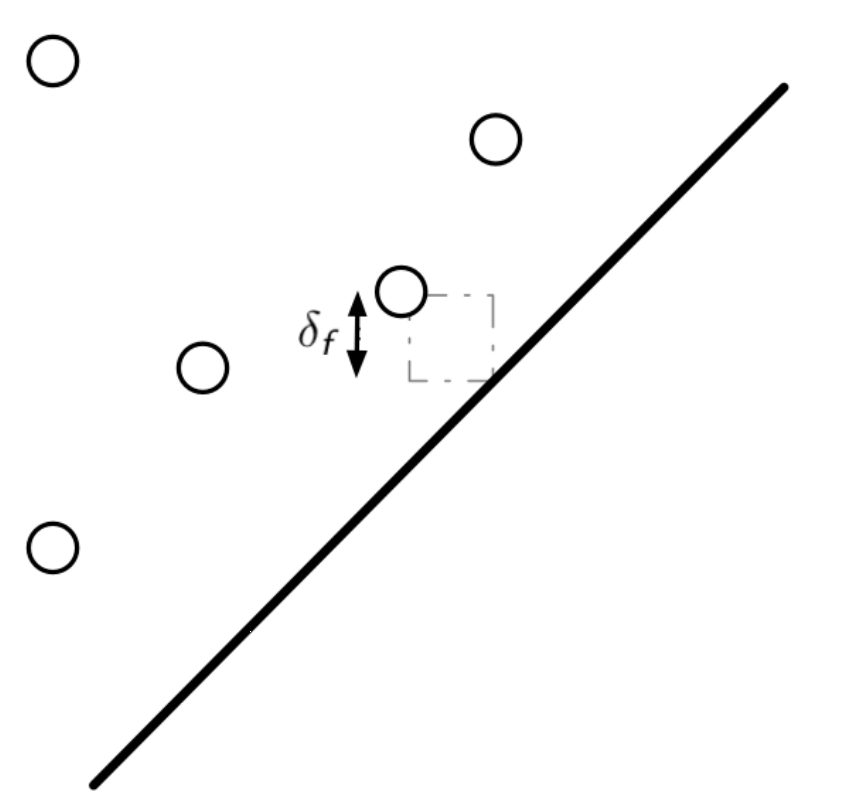
\includegraphics[width=0.35\textwidth]{include/figuras/distanciaDelta.png} 
\caption{Representación de $\delta_f$. Fuente: \cite{presentacionEstabilidad}}
\label{ref:distanciaDeltaF}
\end{figure}

Si dibujamos cuadrados de radio $\epsilon = \delta_f/2$ centrados en los puntos de $\text{Dgm}(f)$, obtenemos una colección de cuadrados disjuntos entre ellos y disjuntos de la diagonal engordada; ver figura \ref{ref:cuadradosF}. Añadiremos otra función tame $g:\mathbb{X} \to \mathbb{R}$ que \emph{es muy cercana a} $f$; ver figura \ref{ref:cuadradosFyG}. Lo que significa que $f$ y $g$ satisfacen que $\norm{f-g}_\infty < \delta_f/2$.

\begin{figure}[!ht]
\centering
\begin{subfigure}{0.4\textwidth}
\centering
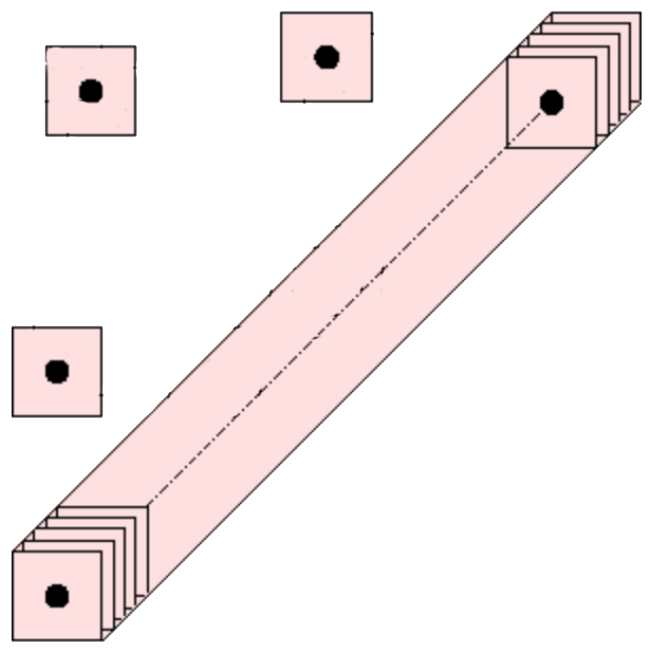
\includegraphics[width=0.6\textwidth]{include/figuras/cuadradosF.png} 
\caption{Cuadrados de radio $\epsilon$ centrados en los puntos de $\text{Dgm}(f)$. Fuente: \cite{presentacionEstabilidad}}
\label{ref:cuadradosF}
\end{subfigure}\hspace{0.1\textwidth}%
\begin{subfigure}{0.4\textwidth}
\centering
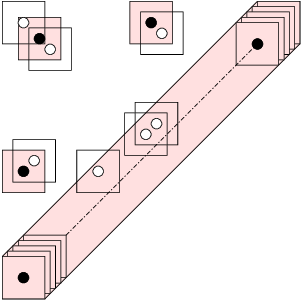
\includegraphics[width=0.6\textwidth]{include/figuras/cuadradosFyG.png} 
\caption{Cuadrados de radio $\epsilon$ centrados en los puntos de $\text{Dgm}(f)$ y $\text{Dgm}(g)$, con $g$ muy cercana a $f$. Fuente: \cite{Cohen-Steiner2007}}
\label{ref:cuadradosFyG}
\end{subfigure}
\caption{}
\end{figure}

Así pues, probaremos el teorema de estabilidad para la distancia bottleneck añadiendo la condición que las funciones tame tienen que \emph{estar muy cerca}.

\begin{lemma}[Lema de la biyección sencilla]
Sean $f,g: \mathbb{X} \to \mathbb{R}$ dos funciones tame, y sea $g$ muy cercana a $f$. Entonces los diagramas de persistencia satisfacen 
\[
W_\infty(\text{\rm Dgm}(f), \text{\rm Dgm}(g)) \leq \norm{f-g}_\infty\,.
\]
\end{lemma}

\begin{proof}
Denotamos $\mu$ a la multiplicidad del punto $p \in (\text{Dgm}(f) \setminus \Delta)$ y $\square_\epsilon$ al cuadrado de centro $p$ y radio $\epsilon = \norm{f-g}_\infty$. Entonces, aplicando el \emph{Lema de la caja} obtenemos que 
\[
\mu = \#(\text{Dgm}(f) \cap \square_0) \leq \#(\text{Dgm}(g) \cap \square_\epsilon) \leq \#(\text{Dgm}(f) \cap \square_{2\epsilon})\,. 
\]

Como $g$ \emph{es muy cercana a} $f$ entonces $\epsilon = \norm{f-g}_\infty < \delta_f/2 \Rightarrow 2\epsilon < \delta_f$. Lo que implica que $p$ es el único punto de $\text{Dgm}(f) \cap \square_{2\epsilon}$, como se puede ver en la figura \ref{ref:biyeccionFacilFig}, por tanto
\[
\#(\text{Dgm}(f) \cap \square_{2\epsilon}) = \mu \Rightarrow \mu \leq \#(\text{Dgm}(g) \cap \square_\epsilon) \leq \mu \Rightarrow \#(\text{Dgm}(g) \cap \square_\epsilon) = \mu\,.
\]

\begin{figure}[!ht]
\centering
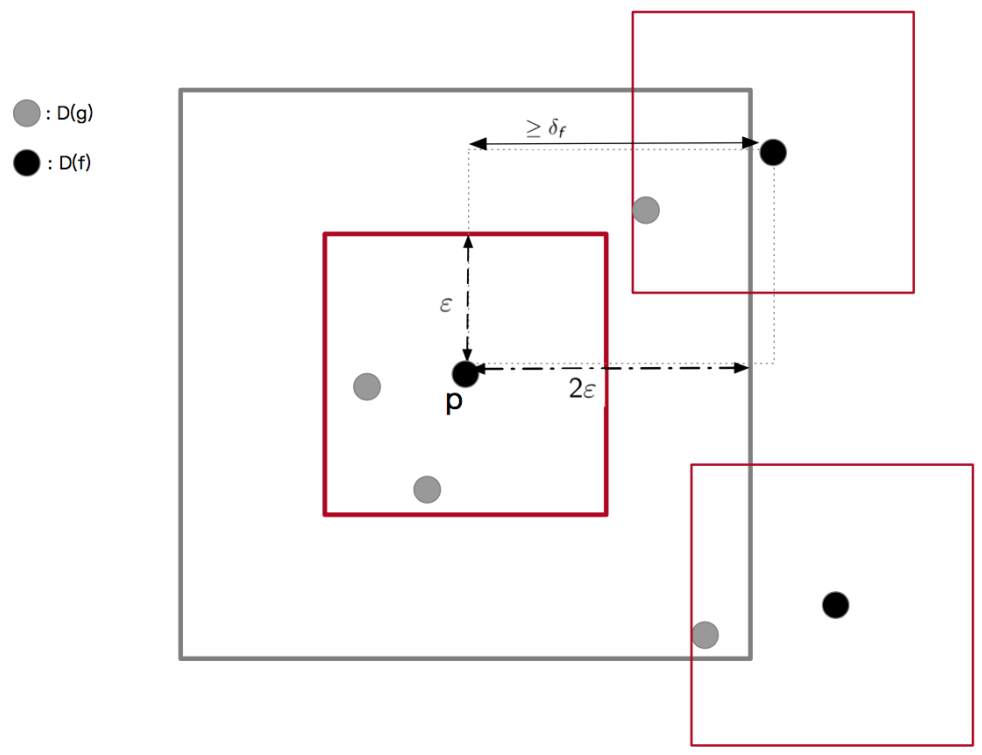
\includegraphics[width=0.75\textwidth]{include/figuras/biyeccionFacilFig.png} 
\caption{Se observa que al ser $g$ \emph{muy cercana a} $f$, entonces $p$ es el único punto de $\text{Dgm}(f) \cap \square_{2\epsilon}$. Fuente: \cite{presentacionEstabilidad}}
\label{ref:biyeccionFacilFig}
\end{figure}

Entonces, podemos emparejar todos los puntos de $\text{Dgm}(g) \cap \square_\epsilon$ a $p$. Repitiendo este proceso para todos los puntos de $\text{Dgm}(f)$ fuera de la diagonal, emparejaremos todos los puntos de $\text{Dgm}(g)$ excepto aquellos que su distancia a $\text{Dgm}(f) \setminus \Delta$ sea mayor que $\epsilon$. Sin embargo, debido a que $H(\text{Dgm}(f), \text{Dgm}(g)) \leq \epsilon$, estos puntos de $\text{Dgm}(g)$ deben estar a distancia menor o igual que $\epsilon$ de la diagonal. Por lo que emparejando estos puntos restantes a su proyección ortogonal sobre la diagonal obtenemos una biyección entre $\text{Dgm}(f)$ y $\text{Dgm}(g)$,  tal y como se muestra en la figura \ref{ref:emparejamientoBiyeccionFacil}.

\begin{figure}[!ht]
\centering
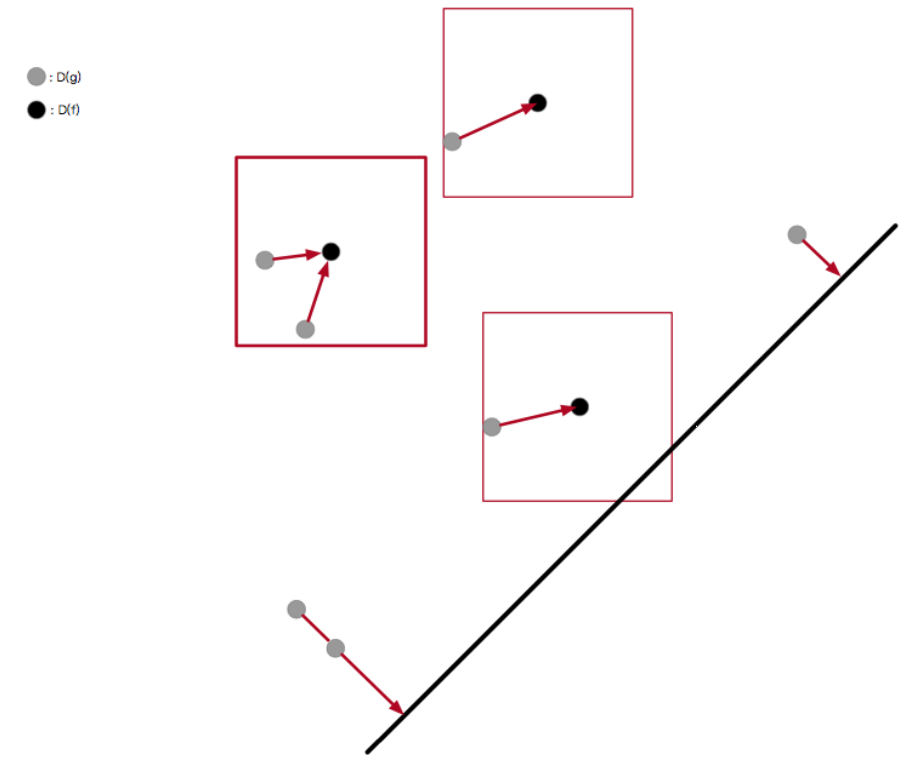
\includegraphics[width=0.75\textwidth]{include/figuras/emparejamientoBiyeccionFacil.png} 
\caption{Emparejamiento de distancia menor que $\epsilon$ entre los puntos de $\text{Dgm}(f)$ y $\text{Dgm}(g)$, para el caso en el que $g$ \emph{es muy cercano a} $f$. Fuente: \cite{presentacionEstabilidad}}
\label{ref:emparejamientoBiyeccionFacil}
\end{figure}

Como la biyección empareja puntos de distancia menor o igual que $\epsilon$, concluimos que la distancia bottleneck entre $\text{Dgm}(f)$ y $\text{Dgm}(g)$ es menor o igual que $\epsilon$.
\end{proof}

\subsubsection*{Estabilidad para la distancia bottleneck con funciones PL}
Nos acercaremos un poco más a la demostración para el caso general, comprobando primero la estabilidad para dos funciones PL $\hat{f}$ y $\hat{g}$ definidas en un complejo simplicial $K$. Recordamos que vimos en la sección \ref{sec:funcionesPL} que las funciones PL eran tame.

Definimos la \emph{combinación convexa} de $\hat{f}$ y $\hat{g}$ como $h_\lambda: (1-\lambda)\hat{f} + \lambda\hat{g}$, para $\lambda \in [0,1]$. Esta familia uniparamétrica de combinaciones convexas forma una interpolación lineal entre las funciones $h_0=\hat{f}$ y $h_1=\hat{g}$.

\begin{lemma}[Lema de la interpolación]
\begin{sloppypar}
Sea $K$ un complejo simplicial y sean ${\hat{f}, \hat{g}: K \to \mathbb{R}}$ dos funciones PL. Entonces,
\end{sloppypar}
\[
W_\infty(\text{\rm Dgm}(\hat{f}), \text{\rm Dgm}(\hat{g})) \leq \norm{\hat{f}-\hat{g}}_\infty\,.
\]
\end{lemma}

\begin{proof}
Descompondremos esta interpolación lineal en suficientes pequeños pasos de forma que podamos usar el \emph{Lema de la biyección sencilla} en cada uno de ellos. Sea $c = \norm{\hat{f}-\hat{g}}_\infty$.

Podemos observar que para que para todo $\lambda \in [0,1]$, $h_\lambda$ es tame y que $\delta(\lambda)=\delta_{h_\lambda}>0$. Para garantizar que $h_\lambda$ es tame veremos que $h_\lambda$ es una función PL. Como $\hat{f}$ y $\hat{g}$ son PL, entonces $\hat{f}(x)= \sum_{i} b_i(x)\hat{f}(u_i)$ y $\hat{g}(x)= \sum_{i} b_i(x)\hat{g}(u_i)$, donde $u_i$ son los vértices de $K$ y $b_i(x)$ son las coordenadas baricéntricas de $x$. Luego,
\begin{gather*}
h_\lambda(x) = (1-\lambda)\hat{f}(x) + \lambda\hat{g}(x)= (1-\lambda)\sum_{i} b_i(x)\hat{f}(u_i) + \lambda \sum_{i} b_i(x)\hat{g}(u_i)=\\
=\sum_{i} b_i(x)\hat{f}(u_i) -\lambda\sum_{i} b_i(x)\hat{f}(u_i) + \lambda \sum_{i} b_i(x)\hat{g}(u_i)=\\
=\sum_{i} b_i(x)((1-\lambda)\hat{f}(u_i)+ \lambda\hat{g}(u_i))\,,
\end{gather*}
por lo que $h_\lambda$ es PL.

Se sigue que el conjunto de los intervalos abiertos $J_\lambda=(\lambda-\delta(\lambda)/4c,\lambda+\delta(\lambda)/4c)\subset \mathbb{R}$ forman un recubrimiento abierto del intervalo $[0,1]$. Como $[0,1]$ es compacto, entonces un subrecubrimiento minimal $C'$ de $C$ será finito. Sean $\lambda_1 < \lambda_2 < ... < \lambda_n$ los puntos medios de los intervalos de $C'$. Como $C'$ es minimal y los intervalos son abiertos, entomces cualquier par de intervalos consecutivos $J_{\lambda_i}$ y $J_{\lambda_{i+1}}$ son no disjuntos. Luego,

\[
\lambda_{i+1} - \lambda_i \leq \dfrac{\delta(\lambda_{i+1}) + \delta(\lambda_{i})}{4c}\leq \dfrac{\max\{\delta(\lambda_{i+1}), \delta(\lambda_{i})\}}{2c}\,.
\]

Por definición de $c$, se cumple que $\norm{h_{\lambda_i}-h_{\lambda_{i+1}}}_\infty =c(\lambda_{i+1} - \lambda_i)$, ya que
\begin{gather*}
\norm{h_{\lambda_i}-h_{\lambda_{i+1}}}_\infty =
\norm{(1-\lambda_i)\hat{f} +\lambda_i\hat{g} - (1-\lambda_{i+1})\hat{f} -\lambda_{i+1}\hat{g}}_\infty =\\
=\norm{(\lambda_{i+1} - \lambda_i)\hat{f} - (\lambda_{i+1} - \lambda_i)\hat{g}}_\infty = 
\abs{\lambda_{i+1} - \lambda_i}\norm{\hat{f}-\hat{g}}_\infty 
=c(\lambda_{i+1} - \lambda_i)\,.
\end{gather*}

Como consecuencia, $\norm{h_{\lambda_i}-h_{\lambda_{i+1}}}_\infty \leq \max\{\delta(\lambda_{i+1}), \delta(\lambda_{i})\}/2$, lo que implica que $h_{\lambda_i}$ \emph{esta muy cercana a} $h_{\lambda_{i+1}}$ o al revés. Por lo que podemos aplicar el \emph{Lema de la biyección sencilla}, el cual nos garantiza que $W_\infty(\text{Dgm}(h_{\lambda_i}), \text{Dgm}(h_{\lambda_i})) \leq \norm{h_{\lambda_i}-h_{\lambda_{i+1}}}_\infty\,$, para todo $1\leq i \leq n-1$. Siendo $\lambda_0=0$ y $\lambda_{n+1}=1$, se sigue dando la desigualdad anterior para $i=0$ e $i=n$, ya que $h_0$ \emph{es muy cercana a} $h_1$ y $h_1$ \emph{es muy cercana a} $h_n$.

Haciendo uso de la \emph{desigualdad triangular de $W_\infty$} obtenemos el resultado,
\begin{gather*}
W_\infty(\text{\rm Dgm}(\hat{f}), \text{\rm Dgm}(\hat{g})) \overset{Des.\ Triang.}{\leq}
\sum_{i=0}^{n} W_\infty(\text{Dgm}(h_{\lambda_i}), \text{Dgm}(h_{\lambda_i})) \leq \sum_{i=0}^{n}\norm{h_{\lambda_i}-h_{\lambda_{i+1}}}_\infty\ =\\
=c\sum_{i=0}^{n}(\lambda_{i+1} - \lambda_i)=c(\lambda_{n+1}-\lambda_0)=c(1-0) = \norm{\hat{f}-\hat{g}}_\infty\,.
\end{gather*}
\end{proof}

\subsubsection*{Estabilidad para la distancia bottleneck con funciones tame}
Tenemos todos los resultados necesarios para poder demostrar el \emph{Teorema de estabilidad para la distancia bottleneck con funciones tame}, el cual recordamos a continuación:

\begin{reptheorem}{th:estabilidadTame}[Teorema de estabilidad para funciones tame]
Sea $\mathbb{X}$ un espacio topológico triangulable y sea $f,g: \mathbb{X} \to \mathbb{R}$ dos funciones tame continuas. Entonces,
\[
W_\infty(\text{\rm Dgm}(f), \text{\rm Dgm}(g)) \leq \norm{f-g}_\infty\,.
\]
\end{reptheorem}

Adicionalmente, necesitaremos recordar un par de nociones de análisis matemático:
\begin{definition}
Dados dos espacios métricos $(X, d_X)$ y $(Y,d_Y)$, y $M \subset X$ entonces una función $f:M \to Y$ se llama \emph{uniformemente continua} en $M$ cuando, para cada $\epsilon > 0$, puede encontrarse $\delta>0$ tal que, si $x_1,x_2 \in M$ verifican que $d_X(x_1,x_2)<\delta$, entonces $d_Y(f(x_1),f(x_2))<\epsilon$.
\end{definition}

\begin{theorem}[Teorema de Heine–Cantor \cite{libroAnalisisMatematico}]
\begin{sloppypar}
Sean $E$ y $F$ espacios métricos y ${f : E \to F}$ una función continua. Si $E$ es compacto, entonces $f$ es uniformemente continua.
\end{sloppypar}
\end{theorem}

\begin{proof}[Demostración del teorema \ref{th:estabilidadTame} (Teorema de estabilidad para funciones tame)]
$ $\newline
Por la definición de espacio triangulable, existe un complejo simplicial (finito) $L$ y un homeomorfismo $\Phi:L \to \mathbb{X}$. Se observa que el diagrama de persistencia es invariante este tipo de cambio de variable, es decir, $f \circ \Phi: L \to \mathbb{R}$ es tame y tiene el mismo diagrama de persistencia que $f$. 

Sea $\delta >0$ lo suficientemente pequeño. Como $f$ y $g$ son continuas, $L$ es compacto, entonces por el \emph{Teorema de Heine-Cantor} $f$ y $g$ son uniformemente compactas, lo que nos garantiza que existe una subdivisión $K$ de $L$ tal que
\begin{gather*}
\abs{f \circ \Phi(u) - f \circ \Phi(v)} \leq \delta\,,\\
\abs{g \circ \Phi(u) - g \circ \Phi(v)} \leq \delta\,,
\end{gather*}
cuando $u$ y $v$ son puntos de un mismo símplice de $K$, ya que podemos obtener esta subdivisión $K$ tal que el diámetro de cada símplice sea tan pequeño como sea necesario para cumplir la condición de la continuidad uniforme de $f$ y $g$.

Sean $\hat{f},\hat{g}:\text{Sd }K \to \mathbb{R}$ las funciones PL que aproximan a $f \circ \Phi$ y $g \circ \Phi$ en $K$. Por construcción de $K$, estas funciones satisfacen $\norm{\hat{f} - f \circ \Phi}_\infty \leq \delta$ y $\norm{\hat{g} - g \circ \Phi}_\infty \leq \delta$.

\begin{sloppypar}
Para terminar utilizaremos la \emph{desigualdad triangular de $W_\infty$} para acotar ${W_\infty(\text{Dgm}(f), \text{Dgm}(g))}$ superiormente por la suma de las distancias entre los diagramas de persistencia de las funciones adyacentes en la secuencia $f, \hat{f}, \hat{g}, g$.
\end{sloppypar}

Para el par $\hat{f}$ y $\hat{g}$ tenemos
\begin{align}
W_\infty(\text{\rm Dgm}(\hat{f}), \text{\rm Dgm}(\hat{g})) 
&\leq \norm{\hat{f}-\hat{g}}_\infty \label{eq:punto1}\\
&\leq \norm{\hat{f} - f \circ \Phi}_\infty + \norm{f \circ \Phi - g \circ \Phi}_\infty + \norm{\hat{g} - g \circ \Phi}_\infty \label{eq:punto2}\\
&\leq \norm{f-g}_\infty +2\delta \label{eq:punto3}
\end{align}

El punto \ref{eq:punto1} se debe al \emph{Lema de la interpolación}, el \ref{eq:punto2} a la \emph{desigualdad triangular de} $d_\infty$ y por último, el punto \ref{eq:punto3} se debe a que $\hat{f}$ y $\hat{g}$ difieren como mucho $\delta$ de $f \circ \Phi$ y $g \circ \Phi$ respectivamente, y que $\norm{f-g}_\infty = \norm{f \circ \Phi - g \circ \Phi}_\infty$.

Para obtener poder acotar la distancia bottleneck entre $f$ y $\hat{f}$, supondremos que $\delta<\delta_f/2$, de forma que podemos aplicar el \emph{Lema de la biyección sencilla}. Como el cambio de variables no afecta al diagrama de persistencia obtenemos que
\[
W_\infty(\text{Dgm}(f), \text{Dgm}(\hat{f}))= 
W_\infty(\text{Dgm}(f \circ \Phi), \text{Dgm}(\hat{f})) \leq \delta\,.  
\]

Análogamente podemos obtener acotar la distancia bottleneck entre $g$ y $\hat{g}$ si asumimos que $\delta < \min\{\delta_f/2,\delta_g/2\}$.

Luego, en total tenemos
\begin{gather*}
W_\infty(\text{Dgm}(f), \text{Dgm}(g)) \overset{Des.\ Triang.}{\leq}\\
\leq W_\infty(\text{Dgm}(f), \text{Dgm}(\hat{f})) + W_\infty(\text{Dgm}(\hat{f}), \text{Dgm}(\hat{g})) + W_\infty(\text{Dgm}(\hat{g}), \text{Dgm}(g)) \leq\\
\leq \norm{f-g}_\infty + 4\delta \underset{\delta \to 0}{\longrightarrow} \norm{f-g}_\infty
\end{gather*}
Como la condición es cierta para todo $\delta > 0$, podemos hacer $\delta$ tan pequeño como queramos. Por tanto queda demostrado el \emph{Teorema de estabilidad}.
\end{proof}


